\documentclass[journal]{IEEEtran}
\usepackage[a5paper, margin=10mm]{geometry}
%\usepackage{lmodern} % Ensure lmodern is loaded for pdflatex
\usepackage{tfrupee} % Include tfrupee package

%iffalse
\let\negmedspace\undefined
\let\negthickspace\undefined
\usepackage{gvv-book}
\usepackage{gvv}
\usepackage{cite}
\usepackage{amsmath,amssymb,amsfonts,amsthm}
\usepackage{algorithmic}
\usepackage{graphicx}
\usepackage{textcomp}
\usepackage{xcolor}
\usepackage{txfonts}
\usepackage{listings}
\usepackage{enumitem}
\usepackage{mathtools}
\usepackage{gensymb}
\usepackage{comment}
\usepackage[breaklinks=true]{hyperref}
\usepackage{tkz-euclide} 
\usepackage{listings}                                        
%\def\inputGnumericTable{}                                 
\usepackage[latin1]{inputenc}                                
\usepackage{color}                                            
\usepackage{array}                                            
\usepackage{longtable}                                       
\usepackage{calc}                                             
\usepackage{multirow}                                         
\usepackage{hhline}                                           
\usepackage{ifthen}                                           
\usepackage{lscape}
\usepackage{tabularx}
\usepackage{array}
\usepackage{float}
\usepackage{multicol}

\newcommand{\BEQA}{\begin{eqnarray}}
\newcommand{\EEQA}{\end{eqnarray}}
%\newcommand{\define}{\stackrel{\triangle}{=}}

\setlength{\headheight}{1cm} % Set the height of the header box
\setlength{\headsep}{0mm}     % Set the distance between the header box and the top of the text


%\usepackage[a5paper, top=10mm, bottom=10mm, left=10mm, right=10mm]{geometry}


\setlength{\intextsep}{10pt} % Space between text and floats

% Marks the beginning of the document
\begin{document}
\onecolumn
\bibliographystyle{IEEEtran}
\vspace{3cm}

%\renewcommand{\theequation}{\theenumi}
\numberwithin{equation}{enumi}
\numberwithin{figure}{enumi}
\renewcommand{\thefigure}{\theenumi}
\renewcommand{\thetable}{\theenumi}

\title{1-1.6-25}
\author{ai24btech11030 - Shiven Bajpai}
\maketitle

\renewcommand{\thefigure}{\theenumi}
\renewcommand{\thetable}{\theenumi}

\textbf{Question: } Three points $P\myvec{h & k}$, $Q\myvec{x_1 & y_1}$ and $R\myvec{x_2 & y_2}$ lie on a line. Show that \begin{align*}\frac{h-x_1}{y_2-y_1} = \frac{k - y_1}{x_2 - x_1}\end{align*}

\textbf{Solution: } Given:
\begin{center}
\begin{tabular}{| c | c | c |}
    \hline
    \textbf{Point} & \textbf{x} & \textbf{y}\\
    \hline
    P & $h$ & $k$\\
    \hline
    Q & $x_1$ & $y_1$\\
    \hline
    R & $x_2$ & $y_2$\\
    \hline
\end{tabular}
\end{center}
    
Since the points P, Q, R are collinear, The matrix $\myvec{P-Q & R-Q}$ must have rank 1.

\begin{align*}
    \myvec{P-Q & R-Q}^T &= \myvec{h-x_1 & x_2 - x_1 \\ y-y_1 & y_2-y_1}\\
    \text{Using  } R_2 &\leftarrow R_2 - \frac{k-y_1}{h-x_1}R_1\\
    &= \myvec{h-x_1 & x_2 - x_1 \\ 0 & y_2-y_1 -\frac{\brak{k-y_1}\brak{{x_2 - x_1}}}{h-x_1}}
\end{align*}

Since matrix has rank 1, we can say

\begin{align*}
    y_2-y_1 -\frac{\brak{k-y_1}\brak{{x_2 - x_1}}}{h-x_1} &= 0\\
    \frac{h-x_1}{y_2-y_1} &= \frac{k - y_1}{x_2 - x_1}
\end{align*}

\newpage

\begin{figure}[H]
	\centering
	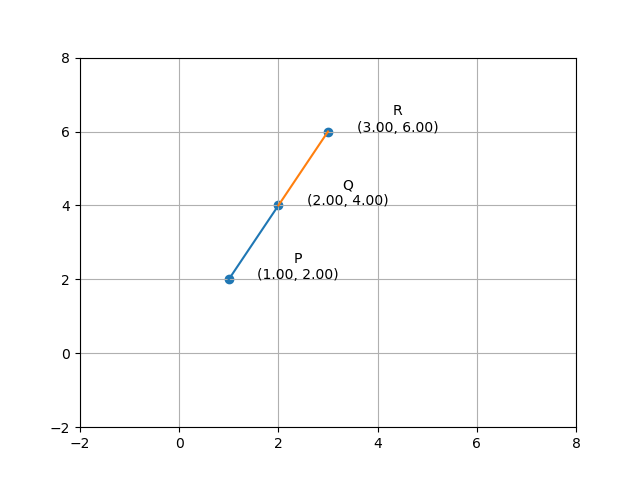
\includegraphics[width=0.75\columnwidth]{Figures/Figure.png}
	\label{fig}
\end{figure}


Console Output:
\begin{verbatim}
/mnt/D/Cl/EE1030/Question_3/Codes$ python3 main.py 
Taking point P to be:
 [[1.]
 [2.]]
Taking point Q to be:
 [[2.]
 [4.]]
Taking point R to be:
 [[3.]
 [6.]]
Calculated LHS to be: 2.0
Calculated RHS to be: 2.0
\end{verbatim}

Code for this plot can be found at:
\begin{lstlisting}
    Codes/main.py
    Codes/main.c
\end{lstlisting}

\end{document}
